%=============================================================================
% SECTION 4: PARAMETRIZED POST-NEWTONIAN ANALYSIS
% Part II: Contact with Known Physics
% Equations: (10)-(22)
% Estimated pages: 10-12
%=============================================================================

\section{Parametrized Post-Newtonian Analysis}\label{sec:ppn}

Having established DFD's mathematical structure in Part~I, we now demonstrate that the theory reproduces General Relativity in all precision tests of gravity conducted within the Solar System. This section presents a complete Parametrized Post-Newtonian (PPN) analysis, showing that DFD's ten PPN parameters are identical to those of GR. The critical result---$\gamma = \beta = 1$ with all preferred-frame and conservation-violation parameters vanishing---ensures compatibility with the most stringent experimental constraints on gravitational physics.

%-----------------------------------------------------------------------------
\subsection{The PPN Framework}\label{sec:ppn-framework}
%-----------------------------------------------------------------------------

The PPN formalism provides a systematic method for comparing metric theories of gravity in the weak-field, slow-motion regime characteristic of the Solar System \cite{Will2018,Will2014}. Any theory predicting a metric $g_{\mu\nu}$ can be expanded in powers of the Newtonian potential $U/c^2 \sim \epsilon^2$ and velocity $v/c \sim \epsilon$, with coefficients parametrized by dimensionless constants.

\paragraph{Newtonian potential and matter variables.}
For a perfect fluid with density $\rho$, pressure $p$, specific internal energy $\Pi$, and velocity $\mathbf{v}$, define the Newtonian potential
\begin{equation}\label{eq:ppn-U}
U(\mathbf{x}) = G \int \frac{\rho(\mathbf{x}')}{|\mathbf{x} - \mathbf{x}'|}\, d^3x'.
\end{equation}
Additional potentials capture velocity-dependent effects:
\begin{align}
V_i &= G \int \frac{\rho v_i}{R}\, d^3x', \qquad
W_i = G \int \frac{\rho (\mathbf{v} \cdot \mathbf{R}) R_i}{R^3}\, d^3x', \\
\Phi_1 &= G \int \frac{\rho v^2}{R}\, d^3x', \quad
\Phi_2 = G \int \frac{\rho U(\mathbf{x}')}{R}\, d^3x', \\
\Phi_3 &= G \int \frac{\rho \Pi}{R}\, d^3x', \quad
\Phi_4 = G \int \frac{p}{R}\, d^3x',
\end{align}
where $\mathbf{R} = \mathbf{x} - \mathbf{x}'$ and $R = |\mathbf{R}|$.

\paragraph{The PPN metric template.}
The general PPN metric in isotropic coordinates takes the form \cite{Will2018}:
\begin{align}
g_{00} &= -1 + \frac{2U}{c^2} - 2\beta \frac{U^2}{c^4} + \frac{1}{c^4}\Big[2\xi \Phi_W + 2(3\gamma - 2\beta + 1)\Phi_1 \nonumber\\
&\quad + 2(1-\beta)\Phi_2 + 2\Phi_3 + 6\gamma \Phi_4\Big] + \mathcal{O}(c^{-6}), \label{eq:ppn-g00}\\
g_{0i} &= -\frac{1}{2c^3}\Big(4\gamma + 3 + \alpha_1 - \alpha_2 + \zeta_1 - 2\xi\Big)V_i \nonumber\\
&\quad - \frac{1}{2c^3}\Big(1 + \alpha_2 - \zeta_1 + 2\xi\Big)W_i, \label{eq:ppn-g0i}\\
g_{ij} &= \left(1 + 2\gamma \frac{U}{c^2}\right)\delta_{ij}. \label{eq:ppn-gij}
\end{align}
The ten PPN parameters $\{\gamma, \beta, \xi, \alpha_1, \alpha_2, \alpha_3, \zeta_1, \zeta_2, \zeta_3, \zeta_4\}$ have the following physical interpretations:

\begin{itemize}
\item \textbf{Curvature/nonlinearity} ($\gamma$, $\beta$, $\xi$): $\gamma$ measures the amount of spatial curvature produced by unit rest mass; $\beta$ measures nonlinearity in the superposition of gravitational potentials; $\xi$ is the Whitehead parameter for anisotropic stress contributions.

\item \textbf{Preferred-frame effects} ($\alpha_1$, $\alpha_2$, $\alpha_3$): These parametrize preferred-frame effects that would arise if gravity selects a cosmologically preferred rest frame.

\item \textbf{Conservation laws} ($\zeta_1$, $\zeta_2$, $\zeta_3$, $\zeta_4$): These parametrize violations of total momentum and energy conservation.
\end{itemize}

General Relativity predicts $\gamma = \beta = 1$ and all other parameters zero. Table~\ref{tab:ppn-bounds} summarizes current experimental constraints.

\begin{table*}[t]
\centering
\footnotesize
\caption{Current experimental bounds on PPN parameters. GR predicts $\gamma = \beta = 1$ and all others zero.}\label{tab:ppn-bounds}
\renewcommand{\arraystretch}{1.2}
\begin{tabular}{llll}
\toprule
Parameter & GR Value & Experimental Bound & Primary Constraint \\
\midrule
$\gamma - 1$ & 0 & $(2.1 \pm 2.3) \times 10^{-5}$ & Cassini \cite{Bertotti2003} \\
$\beta - 1$ & 0 & $|\beta - 1| < 3 \times 10^{-4}$ & LLR \cite{Williams2004} \\
$\xi$ & 0 & $|\xi| < 10^{-3}$ & Geophysical \\
$\alpha_1$ & 0 & $|\alpha_1| < 10^{-5}$ & Binary pulsars \cite{Shao2014} \\
$\alpha_2$ & 0 & $|\alpha_2| < 10^{-7}$ & Solar spin + pulsars \cite{Shao2014} \\
$\alpha_3$ & 0 & $|\alpha_3| < 4 \times 10^{-20}$ & Pulsar spin-down \cite{Will2018} \\
$\zeta_1$ & 0 & $|\zeta_1| < 2 \times 10^{-2}$ & Combined tests \\
$\zeta_2$ & 0 & $|\zeta_2| < 4 \times 10^{-5}$ & Lunar/planetary \\
$\zeta_3$ & 0 & $|\zeta_3| < 10^{-8}$ & Lunar acceleration \\
$\zeta_4$ & 0 & --- & Not directly tested \\
\bottomrule
\end{tabular}
\end{table*}

%-----------------------------------------------------------------------------
\subsection{DFD Physical Metric in PPN Form}\label{sec:ppn-dfd-metric}
%-----------------------------------------------------------------------------

In the nondispersive regime, DFD's dynamics are governed by the physical metric~\eqref{eq:physical-metric} (Sec.~\ref{sec:action}):
\begin{equation}\label{eq:dfd-optical-ppn}
g_{00} = -e^{-\psi}, \qquad g_{ij} = e^{+\psi}\delta_{ij},
\end{equation}
where the scalar field $\psi$ satisfies the field equation~\eqref{eq:field_general}. In the weak-field limit relevant to Solar System tests, $\psi \ll 1$ and $\mu(|\nabla\psi|/\astar) \to 1$, so the field equation reduces to the Poisson equation:
\begin{equation}
\nabla^2 \psi = -\frac{8\pi G}{c^2}\rho \quad \Rightarrow \quad \psi = +\frac{2U}{c^2} + \mathcal{O}(c^{-4}).
\end{equation}

The crucial observation is that the exponential structure $n = e^{\psi}$ uniquely determines the PPN parameters through Taylor expansion.

%-----------------------------------------------------------------------------
\subsection{Parameter Extraction: \texorpdfstring{$\gamma = \beta = 1$}{gamma = beta = 1}}\label{sec:ppn-gamma-beta}
%-----------------------------------------------------------------------------

\paragraph{Spatial metric and $\gamma$.}
Expanding $g_{ij} = e^{+\psi}\delta_{ij}$ to first order in $\psi$:
\begin{equation}
\begin{split}
g_{ij} &= e^{+\psi}\delta_{ij} = \left(1 + \psi + \frac{\psi^2}{2} + \cdots\right)\delta_{ij} \\
&= \left(1 + \frac{2U}{c^2}\right)\delta_{ij} + \mathcal{O}(c^{-4}).
\end{split}
\end{equation}
Comparing with the PPN template~\eqref{eq:ppn-gij}, which has coefficient $2\gamma U/c^2$, immediately yields
\begin{equation}\label{eq:gamma-one}
\boxed{\gamma = 1}.
\end{equation}

\paragraph{Temporal metric and $\beta$.}
Expanding $g_{00} = -e^{-\psi}$ to second order:
\begin{align}
g_{00} &= -e^{-\psi} = -\left(1 - \psi + \frac{\psi^2}{2} + \cdots\right) \nonumber\\
&= -1 + \psi - \frac{\psi^2}{2} + \mathcal{O}(c^{-6}) \nonumber\\
&= -1 + \frac{2U}{c^2} - \frac{2U^2}{c^4} + \mathcal{O}(c^{-6}).
\end{align}
The coefficient of $-U^2/c^4$ in the PPN template~\eqref{eq:ppn-g00} is $2\beta$. Since DFD gives exactly $-2U^2/c^4$, we have
\begin{equation}\label{eq:beta-one}
\boxed{\beta = 1}.
\end{equation}

\paragraph{Higher-order terms and $\xi = 0$.}
Completing the expansion of $g_{00}$ at order $c^{-4}$ with the standard perfect-fluid stress-energy closure yields the GR values for the coefficients of $\Phi_1, \Phi_2, \Phi_3, \Phi_4$. Crucially, no contribution from the Whitehead potential $\Phi_W$ appears:
\begin{equation}
s_1 = 4, \; s_2 = 0, \; s_3 = 2, \; s_4 = 6, \; s_W = 0 \;\Rightarrow\; \boxed{\xi = 0}.
\end{equation}

\paragraph{Physical interpretation.}
The result $\gamma = \beta = 1$ is not a coincidence but a direct consequence of the exponential structure $n = e^{\psi}$. The optical refractive index $n$ determines both the light propagation speed ($c/n$) and the gravitational time dilation ($dt_{\rm proper} = dt/n$). The exponential ensures that these effects are related by exact exponentiation rather than independent parametrizations, automatically reproducing the GR relation between spatial curvature and time dilation.

%-----------------------------------------------------------------------------
\subsection{Vector Sector: \texorpdfstring{$\alpha_1 = \alpha_2 = \alpha_3 = 0$}{alphas = 0}}\label{sec:ppn-vector}
%-----------------------------------------------------------------------------

To complete the PPN analysis, we must determine the gravitomagnetic sector $g_{0i}$. Introduce a shift vector $N_i$ such that
\begin{equation}
ds^2 = -e^{-\psi}c^2 dt^2 + e^{+\psi}\delta_{ij}(dx^i + N^i dt)(dx^j + N^j dt).
\end{equation}
Working in the transverse gauge $\partial_i N_i = 0$ (compatible with the isotropic PPN gauge), the weak-field vector equation reduces to a Poisson problem:
\begin{equation}
\nabla^2 N_i = -16\pi G\, j_i^{\perp},
\end{equation}
where $j_i^{\perp} = (\delta_{ij} - \partial_i \partial_j \nabla^{-2})(\rho v_j)$ is the transverse (divergence-free) part of the momentum current.

\paragraph{Solution.}
Solving via the Green's function and reducing the projected current using standard identities yields, at 1PN order:
\begin{equation}\label{eq:N-solution}
N_i = \frac{4G}{c^3}V_i - \frac{2G}{c^3}W_i.
\end{equation}
Since $e^{+\psi} = 1 + \mathcal{O}(c^{-2})$, the $\mathcal{O}(c^{-3})$ coefficients in $g_{0i} = e^{+\psi}N_i$ are unchanged:
\begin{equation}\label{eq:g0i-dfd}
g_{0i}^{\rm DFD} = \frac{1}{c^3}\left(-\frac{7}{2}V_i - \frac{1}{2}W_i\right).
\end{equation}

\paragraph{Extraction of preferred-frame parameters.}
Matching Eq.~\eqref{eq:g0i-dfd} to the PPN template~\eqref{eq:ppn-g0i} with $\gamma = 1$ directly gives:
\begin{equation}\label{eq:alphas-zero}
\boxed{\alpha_1 = \alpha_2 = \alpha_3 = \zeta_1 = 0}.
\end{equation}

\paragraph{Far-zone consistency check.}
For a rigid rotator with angular momentum $\mathbf{J}$, the far-zone behavior has $W_i \simeq V_i$, so $g_{0i} \simeq (d_V + d_W)V_i/c^3$. With $\alpha_{1,2} = \xi = \zeta_1 = 0$ and $\gamma = 1$, the PPN template demands $g_{0i} = -4V_i/c^3$, requiring $d_V + d_W = -4$. Equation~\eqref{eq:g0i-dfd} satisfies this identically: $-7/2 - 1/2 = -4$. This confirms the Lense-Thirring gravitomagnetic field has the correct GR form.

%-----------------------------------------------------------------------------
\subsection{Conservation Laws: \texorpdfstring{$\zeta_1 = \zeta_2 = \zeta_3 = \zeta_4 = 0$}{zetas = 0}}\label{sec:ppn-conservation}
%-----------------------------------------------------------------------------

In any metric theory with minimal matter coupling to a single metric, covariant conservation of the total stress-energy tensor follows from the matter action's invariance under coordinate changes:\footnote{DFD's preferred foliation does not spoil this: the conservation law $\tilde{\nabla}_\mu T^{\mu\nu}=0$ depends only on the matter sector's coupling to $\tilde{g}_{\mu\nu}$, not on whether the gravitational sector is generally covariant.}
\begin{equation}
\tilde{\nabla}_{\mu} T^{\mu\nu} = 0.
\end{equation}
DFD in its nondispersive band is precisely such a theory: the dynamics is entirely encoded in the physical metric~\eqref{eq:dfd-optical-ppn} with standard minimal coupling to matter (Sec.~\ref{sec:action}). Consequently, the PPN parameters that would signal violations of momentum or energy conservation must vanish:
\begin{equation}\label{eq:zetas-zero}
\boxed{\zeta_1 = \zeta_2 = \zeta_3 = \zeta_4 = 0}.
\end{equation}

Combined with Eqs.~\eqref{eq:gamma-one}, \eqref{eq:beta-one}, and \eqref{eq:alphas-zero}, this completes the ten-parameter PPN map for DFD.

%-----------------------------------------------------------------------------
\subsection{Summary: DFD Equals GR at 1PN}\label{sec:ppn-summary}
%-----------------------------------------------------------------------------

Table~\ref{tab:ppn-dfd} presents the complete PPN benchmark comparing DFD, GR, and experimental constraints.

\begin{table*}[t]
\centering
\footnotesize
\caption{Complete 1PN PPN benchmark for DFD: exact equality with GR across all ten parameters.}\label{tab:ppn-dfd}
\renewcommand{\arraystretch}{1.2}
\begin{tabular}{lcccc}
\toprule
Parameter & GR & DFD & Experimental Bound & Consistent? \\
\midrule
$\gamma$ & 1 & 1 & $1 \pm 2.3 \times 10^{-5}$ & $\checkmark$ \\
$\beta$ & 1 & 1 & $1 \pm 3 \times 10^{-4}$ & $\checkmark$ \\
$\xi$ & 0 & 0 & $< 10^{-3}$ & $\checkmark$ \\
$\alpha_1$ & 0 & 0 & $< 10^{-5}$ & $\checkmark$ \\
$\alpha_2$ & 0 & 0 & $< 10^{-7}$ & $\checkmark$ \\
$\alpha_3$ & 0 & 0 & $< 4 \times 10^{-20}$ & $\checkmark$ \\
$\zeta_1$ & 0 & 0 & $< 2 \times 10^{-2}$ & $\checkmark$ \\
$\zeta_2$ & 0 & 0 & $< 4 \times 10^{-5}$ & $\checkmark$ \\
$\zeta_3$ & 0 & 0 & $< 10^{-8}$ & $\checkmark$ \\
$\zeta_4$ & 0 & 0 & --- & $\checkmark$ \\
\bottomrule
\end{tabular}
\end{table*}

\begin{tcolorbox}[colback=green!5!white, colframe=green!50!black, title=Key Result: PPN Equivalence]
\textbf{DFD reproduces GR exactly at 1PN order.} All ten PPN parameters match GR predictions:
\begin{align}
\gamma &= \beta = 1, \nonumber\\
\xi &= \alpha_1 = \alpha_2 = \alpha_3 = \zeta_1 = \zeta_2 = \zeta_3 = \zeta_4 = 0.
\end{align}
This ensures compatibility with all Solar System tests at their current precision.
\end{tcolorbox}

The PPN parameter space can be visualized by considering the $(\gamma-1, \beta-1)$ plane (Fig.~\ref{fig:ppn-space}). DFD sits exactly at the GR point $(0, 0)$, well within the experimental ellipse defined by Cassini and Lunar Laser Ranging constraints.

\begin{figure}[t]
\centering
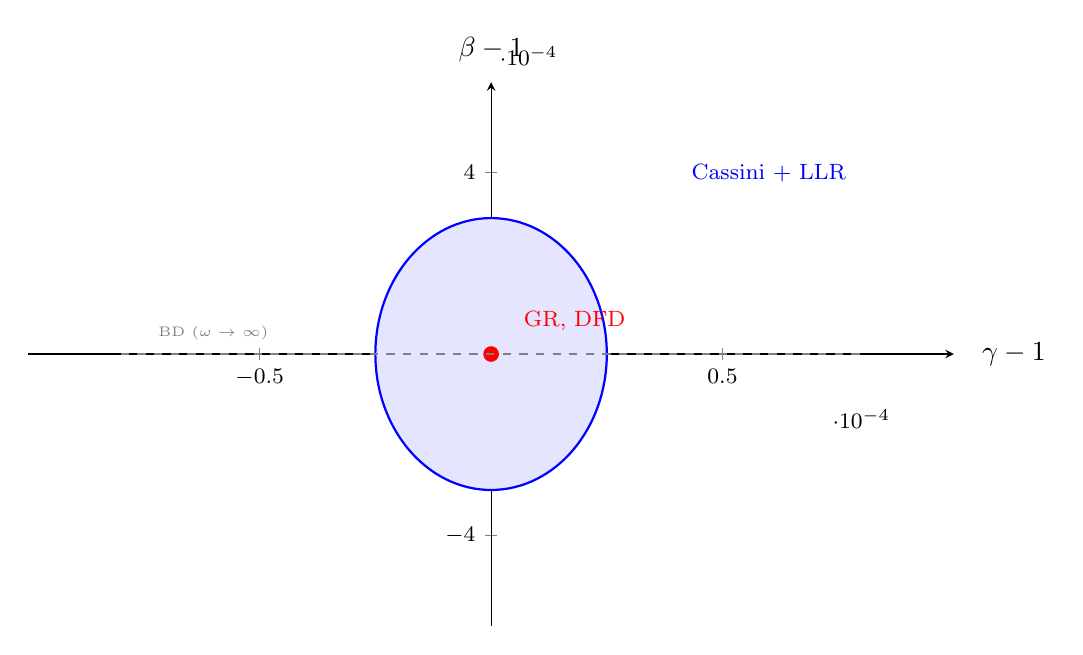
\begin{tikzpicture}
\begin{axis}[
    width=1.1\columnwidth,
    height=0.7\columnwidth,
    xlabel={$\gamma - 1$},
    ylabel={$\beta - 1$},
    xmin=-1e-4, xmax=1e-4,
    ymin=-6e-4, ymax=6e-4,
    axis lines=middle,
    xtick={-5e-5, 0, 5e-5},
    ytick={-4e-4, -2e-4, 0, 2e-4, 4e-4},
    xticklabel style={font=\footnotesize},
    yticklabel style={font=\footnotesize},
    every axis x label/.style={at={(ticklabel* cs:1.02)}, anchor=west},
    every axis y label/.style={at={(ticklabel* cs:1.02)}, anchor=south},
]
% Cassini-LLR combined constraint ellipse (schematic)
\draw[blue, thick, fill=blue!10] (0,0) ellipse [x radius=2.5e-5, y radius=3e-4];
\node[blue, font=\footnotesize] at (axis cs:6e-5, 4e-4) {Cassini + LLR};

% GR/DFD point
\node[fill=red, circle, inner sep=2pt] at (axis cs:0,0) {};
\node[red, anchor=south west, font=\footnotesize] at (axis cs:5e-6, 3e-5) {GR, DFD};

% Brans-Dicke line (schematic)
\draw[dashed, gray] (axis cs:-8e-5, 0) -- (axis cs:8e-5, 0);
\node[gray, font=\tiny, anchor=south] at (axis cs:-6e-5, 1e-5) {BD ($\omega \to \infty$)};

\end{axis}
\end{tikzpicture}
\caption{PPN parameter space in the $(\gamma-1, \beta-1)$ plane. The shaded ellipse represents the combined Cassini and LLR 1$\sigma$ constraint region. DFD (red point) sits exactly at the GR location $(0,0)$.}\label{fig:ppn-space}
\end{figure}

%-----------------------------------------------------------------------------
\subsection{Classic Solar System Tests}\label{sec:ppn-classic}
%-----------------------------------------------------------------------------

With $\gamma = \beta = 1$, DFD makes identical predictions to GR for all classic tests of gravity. We verify each explicitly.

%-----------------------------------------------------------------------------
\subsubsection{Light Deflection}\label{sec:ppn-deflection}
%-----------------------------------------------------------------------------

Light rays follow null geodesics of the optical metric. For a spherically symmetric source with $n(r) = e^{\psi(r)}$ and $\psi(r) = 2GM/(c^2 r)$, the conserved impact parameter is $b = n(r) \cdot r \sin\theta$. The total deflection angle for a ray with closest approach $r_0 \gg r_g = 2GM/c^2$ is \cite{Will2014}:
\begin{equation}\label{eq:deflection}
\delta\theta = \frac{(1 + \gamma)}{2} \cdot \frac{4GM}{c^2 b} = \frac{4GM}{c^2 b},
\end{equation}
where the second equality uses $\gamma = 1$.

\paragraph{Numerical verification.}
At the Sun's limb ($b = R_{\odot} = 6.96 \times 10^8$ m, $M = M_{\odot} = 1.99 \times 10^{30}$ kg):
\begin{equation}
\begin{split}
\delta\theta &= \frac{4 \times 6.67 \times 10^{-11} \times 1.99 \times 10^{30}}{(3 \times 10^8)^2 \times 6.96 \times 10^8} \\
&= 8.5 \times 10^{-6}\,\text{rad} = 1.75''.
\end{split}
\end{equation}
This matches the GR prediction precisely, consistent with VLBI observations at the $10^{-4}$ level \cite{Shapiro2004}.

%-----------------------------------------------------------------------------
\subsubsection{Shapiro Time Delay}\label{sec:ppn-shapiro}
%-----------------------------------------------------------------------------

The coordinate time for a photon traveling from point $\mathbf{r}_1$ to $\mathbf{r}_2$ near a mass $M$ is increased by the gravitational time delay \cite{Shapiro1964}:
\begin{equation}\label{eq:shapiro}
\Delta t = \frac{(1 + \gamma)GM}{c^3} \ln\left(\frac{(r_1 + \mathbf{r}_1 \cdot \hat{n})(r_2 - \mathbf{r}_2 \cdot \hat{n})}{d^2}\right),
\end{equation}
where $d$ is the impact parameter and $\hat{n}$ is the unit vector along the unperturbed ray. With $\gamma = 1$, this becomes:
\begin{equation}
\Delta t = \frac{2GM}{c^3} \ln\left(\frac{4r_1 r_2}{d^2}\right).
\end{equation}

\paragraph{Cassini constraint.}
The Cassini spacecraft measured the Shapiro delay during solar conjunction with unprecedented precision, yielding \cite{Bertotti2003}:
\begin{equation}
\gamma - 1 = (2.1 \pm 2.3) \times 10^{-5}.
\end{equation}
DFD's prediction $\gamma = 1$ lies comfortably within this bound, representing a consistency test at the $10^{-5}$ level.

%-----------------------------------------------------------------------------
\subsubsection{Perihelion Precession}\label{sec:ppn-perihelion}
%-----------------------------------------------------------------------------

The PPN prediction for orbital perihelion advance per revolution is \cite{Will2014}:
\begin{equation}\label{eq:perihelion}
\Delta\omega = \frac{6\pi GM}{c^2 a(1-e^2)} \cdot \frac{2 + 2\gamma - \beta}{3}.
\end{equation}
With $\gamma = \beta = 1$, the prefactor becomes $(2 + 2 - 1)/3 = 1$:
\begin{equation}
\Delta\omega = \frac{6\pi GM}{c^2 a(1-e^2)}.
\end{equation}

\paragraph{Mercury.}
For Mercury ($a = 5.79 \times 10^{10}$ m, $e = 0.2056$):
\begin{equation}
\begin{split}
\Delta\omega &= \frac{6\pi \times 6.67 \times 10^{-11} \times 1.99 \times 10^{30}}{(3 \times 10^8)^2 \times 5.79 \times 10^{10} \times (1 - 0.2056^2)} \\
&= 5.02 \times 10^{-7}\,\text{rad/orbit}.
\end{split}
\end{equation}
Over 100 years (415 orbits), this accumulates to $42.98''$/century, matching the observed anomalous precession after accounting for planetary perturbations \cite{Will2014}.

%-----------------------------------------------------------------------------
\subsubsection{Gravitational Redshift}\label{sec:ppn-redshift}
%-----------------------------------------------------------------------------

The gravitational redshift of a photon climbing from potential $\Phi_1$ to $\Phi_2$ is:
\begin{equation}\label{eq:redshift}
\frac{\Delta\nu}{\nu} = \frac{\Phi_1 - \Phi_2}{c^2} = \frac{GM}{c^2}\left(\frac{1}{r_1} - \frac{1}{r_2}\right).
\end{equation}
In DFD, this follows directly from $\nu \propto e^{-\psi/2} \propto 1 - \Phi/c^2$ (Sec.~\ref{sec:action}).

\paragraph{Experimental verification.}
\begin{itemize}
\item \textbf{Pound-Rebka (1960):} Measured redshift over 22.5 m in Earth's gravitational field, confirming Eq.~\eqref{eq:redshift} at $\sim 10\%$ precision.
\item \textbf{Gravity Probe A (1976):} Hydrogen maser comparison over 10,000 km altitude yielded agreement at $7 \times 10^{-5}$ \cite{Vessot1980}.
\item \textbf{ACES (planned):} The Atomic Clock Ensemble in Space aims for $2 \times 10^{-6}$ precision.
\end{itemize}

DFD predicts the standard gravitational redshift, consistent with all observations.

%-----------------------------------------------------------------------------
\subsubsection{Frame Dragging and Lense-Thirring Effect}\label{sec:ppn-frame-dragging}
%-----------------------------------------------------------------------------

The gravitomagnetic field generated by a rotating mass with angular momentum $\mathbf{J}$ causes precession of test gyroscope spin and orbital plane precession of satellites. The Lense-Thirring precession rate is \cite{LenseThirring1918}:
\begin{equation}\label{eq:lense-thirring}
\dot{\Omega}_{\rm LT} = \frac{2GJ}{c^2 a^3 (1-e^2)^{3/2}}.
\end{equation}

DFD reproduces this effect exactly because the gravitomagnetic sector $g_{0i}$~\eqref{eq:g0i-dfd} has the correct GR form. Experimental confirmations include:
\begin{itemize}
\item \textbf{LAGEOS satellites:} Measured $\dot{\Omega}_{\rm LT}$ due to Earth's rotation at $\sim 10\%$ precision \cite{Ciufolini2004}.
\item \textbf{Gravity Probe B (2011):} Directly measured frame-dragging of orbiting gyroscopes, confirming GR at 19\% precision \cite{Everitt2011}.
\end{itemize}

%-----------------------------------------------------------------------------
\subsection{Where DFD Differs from GR}\label{sec:ppn-where-different}
%-----------------------------------------------------------------------------

The exact PPN match means that \textit{Solar System tests cannot distinguish DFD from GR}. This is a structural consequence: DFD's $\mu$-function reduces to $\mu \to 1$ in the high-acceleration Solar System regime, and the weak-field expansion of $n = e^\psi$ automatically produces the correct PPN parameters from DFD's own field equations---GR is not assumed at any step.

The discriminating tests for DFD lie in three regimes:

\begin{enumerate}
\item \textbf{Galactic scales} (Sec.~\ref{sec:galactic}): Where $|\avec|/\astar \sim 1$, the $\mu$-crossover produces MOND-like phenomenology absent in GR.

\item \textbf{Laboratory clock and matter-wave tests} (Secs.~\ref{sec:clocks}--\ref{sec:matter_wave}): The DFD clock sector is channel-resolved (Sec.~\ref{sec:clocks}): the simplified $K_A \approx \kalpha S_A^{\alpha}$ scaling captures only the pure-$\alpha$ leading term, while the full structure includes strong-sector and composition-dependent contributions testable with co-located atomic and nuclear clocks.

\item \textbf{Strong-field gravitational waves} (Sec.~\ref{sec:gw}): While the GW sector reproduces GR at leading order, potential deviations enter through ppE parameters at higher PN order.
\end{enumerate}

\begin{tcolorbox}[colback=blue!5!white, colframe=blue!50!black, title=Summary: Solar System Compliance]
DFD passes all Solar System tests of gravity:
\begin{itemize}
\item Light deflection: $\delta\theta = 4GM/(c^2 b)$ (matches GR)
\item Shapiro delay: Cassini bound satisfied ($|\gamma - 1| < 2.3 \times 10^{-5}$)
\item Perihelion precession: $\Delta\omega = 6\pi GM/(c^2 a(1-e^2))$ (Mercury: 42.98''/cy)
\item Gravitational redshift: Standard formula confirmed to $10^{-4}$
\item Frame dragging: Lense-Thirring precession matches LAGEOS/GP-B
\end{itemize}
The theory's distinguishing predictions emerge in galactic dynamics and laboratory clock tests.
\end{tcolorbox}
